\section{Dynamics in Asymmetric Staircase Circuits} \label{sec:stairs}

We can use the tools from the previous section to analyze the asymmetry of information speeds in various quantum circuits. First, though, we need to build an asymmetric circuit. There are a few possibilities. The circuits could have 3-site unitary operators, with the gates chosen so that their dynamics are asymmetric. An example gate would be the 3-site swap discussed earlier. Alternatively, we could change the probabilities of gates falling on sites so that if a gate falls across bond $x$, the next gate is more likely to fall across bond $x+r$ for small $r$. This would lead to correlations in gate locations.

The architecture considered in this section will be a limiting case of correlated gates. We will again use the solvable large-$q$ limit. Gates will fall in sets of $n$. Each $n$ gates will fall consecutively across bonds $x, x+1\dots x+n-1$. The first site of each staircase is chosen randomly. These sets of gates are called staircases, and when the bond location is increasing it is called a right staircase. If there are $n$ gates in a staircase it is called an $n$-stair. They are called staircases because using the surface growth picture in Fig.~\ref{fig:tetris} they look like steps, as in Fig.~\ref{fig:stairs}. 
\begin{figure}
	\centering
	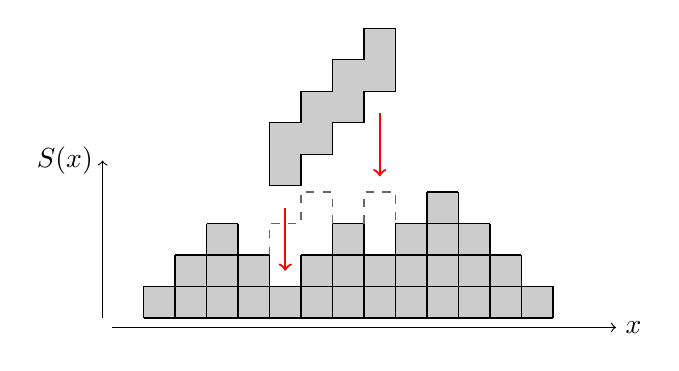
\begin{tikzpicture}[scale = .4]
\draw[->] (0, -.3) -- (16,-.3) node[right]{$x$};
\draw[->] (-.3,0) -- (-.3,5) node[left]{$S(x)$};
\fill[black!20] (1,0) -- (1,1) -- (2,1) -- (2,2) -- (3,2) -- (3,3) -- 
     			(4,3) -- (4,2) -- (5,2) -- (5,1) -- (6,1) -- (6,2) -- (7,2) -- (7,3) -- (8,3) -- (8,2) -- (9,2) -- (9,3) -- (10,3) -- (10,4) 
     			 -- (11,4) -- (11,3) -- (12,3) -- (12,2) -- (13,2) -- (13,1)  -- (14,1) -- (14,0);
     			 
\draw (1,0) -- (14,0);
\draw (1,1) -- (14,1);
\draw (2,2) -- (5,2);
\draw (6,2) -- (13,2);
\draw (3,3) -- (4,3);
\draw (7,3) -- (8,3);
\draw (9,3) -- (12,3);
\draw (10,4) -- (11,4);
\draw (1,0) -- (1,1);
\draw (2,0) -- (2,2);
\draw (3,0) -- (3,3);
\draw (4,0) -- (4,3);
\draw (5,0) -- (5,2);
\draw (6,0) -- (6,2);
\draw (7,0) -- (7,3);
\draw (8,0) -- (8,3);
\draw (9,0) -- (9,3);
\draw (10,0) -- (10,4);
\draw (11,0) -- (11,4);
\draw (12,0) -- (12,3);
\draw (13,0) -- (13,2);
\draw (14,0) -- (14,1);

\draw[fill=black!20] (5,5.2) -- (5,4.2) -- (6,4.2) -- (6,5.2) -- (7,5.2) --  
                     (7,6.2) --
					 (8,6.2) -- (8,7.2) -- (9,7.2) -- (9,8.2) -- (9,9.2) -- (8,9.2)
					 -- (8,8.2) -- (7,8.2) -- (7,7.2) -- (6,7.2) -- (6,6.2) -- (5,6.2)
					 -- (5,5.2);
\draw[thick, ->, red] (5.5,3.5) -- (5.5,1.5);
\draw[thick, ->, red] (8.5,6.5) -- (8.5,4.5);

\draw[dashed, black!60] (5,2) -- (5,3) -- (6,3) -- (6,4) -- (7,4) -- (7,3);
\draw[dashed, black!60] (8,3) -- (8,4) -- (9,4) -- (9,3);
\end{tikzpicture}
%\begin{tikzpicture}[scale = .3, cross/.style={path picture={ 
%		\draw[black]
%		(path picture bounding box.south east) -- (path picture bounding box.north west) (path picture bounding box.south west) -- (path picture bounding box.north east);
%}}]
%
%\draw[->] (0, -.3) -- (16,-.3) node[right]{$x$};
%\draw[->] (-.3,0) -- (-.3,5) node[left]{$S(x)$};
%\fill[black!20] (0,0) -- (3,3) -- (5,1) -- (7,3) -- (8,2) --
%(10,4) -- (14,0) ;
%\draw (0,0) -- (3,3);
%\draw (2,0) -- (4,2);
%\draw (4,0) -- (7,3);
%\draw (6,0) -- (10,4);
%\draw (8,0) -- (11,3);
%\draw (10,0) -- (12,2);
%\draw (12,0) -- (13,1);
%\draw (2,0) -- (1,1);
%\draw (4,0) -- (2,2);
%\draw (6,0) -- (3,3);
%\draw (8,0) -- (6,2);
%\draw (10,0) -- (7,3);
%\draw (12,0) -- (9,3);
%\draw (14,0) -- (10,4);
%\draw[dashed, black!60]  (5,3) -- (6,4);
%\draw[dashed, black!60]  (7,3) -- (6,4);
%\draw[dashed, black!60]  (6,2) -- (5,3);
%
%\draw[fill=black!20] (5,6) -- (6,5) -- (7,6) -- (6,7) -- (5,6);
%\draw[thick, ->, red] (6,4.5) -- (6,3);
%%\node [draw,circle,cross,minimum width=1](B) at (6,3.5){}; 
%\end{tikzpicture}

	\caption{\textbf{Staircase circuit architecture,} in which the gate at site $x$ is always followed by ones at sites $x+1, x+2$, and $x+3$ making this a 4-stair. Note that not all gates are productive, only the ones that fall on sites that are local minima when they fall.}
	\label{fig:stairs}
\end{figure}
In the picture in which the entropy has slope up or down at each site, as in Fig.~\ref{fig:diaggate}, $n$-stair look like $n\times 1$ rectangles tilted $45^\circ$, as in Fig.~\ref{fig:diagstairs}.
\begin{figure}
	\centering
	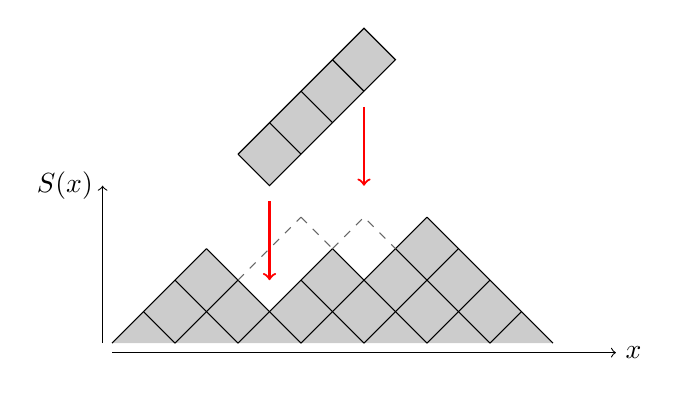
\begin{tikzpicture}[scale = .4]
\draw[->] (0, -.3) -- (16,-.3) node[right]{$x$};
\draw[->] (-.3,0) -- (-.3,5) node[left]{$S(x)$};
\fill[black!20] (0,0) -- (3,3) -- (5,1) -- (7,3) -- (8,2) --
				(10,4) -- (14,0) ;
\draw (0,0) -- (3,3);
\draw (2,0) -- (4,2);
\draw (4,0) -- (7,3);
\draw (6,0) -- (10,4);
\draw (8,0) -- (11,3);
\draw (10,0) -- (12,2);
\draw (12,0) -- (13,1);
\draw (2,0) -- (1,1);
\draw (4,0) -- (2,2);
\draw (6,0) -- (3,3);
\draw (8,0) -- (6,2);
\draw (10,0) -- (7,3);
\draw (12,0) -- (9,3);
\draw (14,0) -- (10,4);

\draw[fill=black!20] (4,6) -- (5,5) -- (6,6) -- (7,7) -- (8,8) -- (9,9) --
					 (8,10) -- (7,9) -- (6,8) -- (5,7) -- (4,6);
\draw (6,6) -- (5,7);
\draw (7,7) -- (6,8);
\draw (8,8) -- (7,9);
%\draw (9,9) -- ()
\draw[thick, ->, red] (5,4.5) -- (5,2);
\draw[thick, ->, red] (8,7.5) -- (8,5);

\draw[dashed, black!60] (4,2) -- (6,4);
\draw[dashed, black!60] (6,4) -- (7,3);
\draw[dashed, black!60] (7,3) -- (8,4) -- (9,3);
\end{tikzpicture}
%\begin{tikzpicture}[scale = .3, cross/.style={path picture={ 
%		\draw[black]
%		(path picture bounding box.south east) -- (path picture bounding box.north west) (path picture bounding box.south west) -- (path picture bounding box.north east);
%}}]
%
%\draw[->] (0, -.3) -- (16,-.3) node[right]{$x$};
%\draw[->] (-.3,0) -- (-.3,5) node[left]{$S(x)$};
%\fill[black!20] (0,0) -- (3,3) -- (5,1) -- (7,3) -- (8,2) --
%(10,4) -- (14,0) ;
%\draw (0,0) -- (3,3);
%\draw (2,0) -- (4,2);
%\draw (4,0) -- (7,3);
%\draw (6,0) -- (10,4);
%\draw (8,0) -- (11,3);
%\draw (10,0) -- (12,2);
%\draw (12,0) -- (13,1);
%\draw (2,0) -- (1,1);
%\draw (4,0) -- (2,2);
%\draw (6,0) -- (3,3);
%\draw (8,0) -- (6,2);
%\draw (10,0) -- (7,3);
%\draw (12,0) -- (9,3);
%\draw (14,0) -- (10,4);
%%\draw[dashed, black!60]  (5,3) -- (6,4);
%%\draw[dashed, black!60]  (7,3) -- (6,4);
%%\draw[dashed, black!60]  (6,2) -- (5,3);
%
%\draw[fill=black!20] (5,6) -- (6,5) -- (7,6) -- (6,7) -- (5,6);
%\draw[thick, ->, red] (6,4.5) -- (6,3);
%%\node [draw,circle,cross,minimum width=1](B) at (6,3.5){}; 
%\end{tikzpicture}

	\caption{\textbf{Another picture of the staircase architecture.} Note that this picture results in the same final state as in Fig.~\ref{fig:stairs}.}
	\label{fig:diagstairs}
\end{figure}
Since each staircase consists of multiple gates, there is an ambiguity in whether the rate $\gamma$ defines the number of gates per bond per time step or the number of staircases. We will use the convention that it is the number of gates per bond per unit time, so that $\gamma/n$ is the rate of staircases.

Ref.~\cite{Nahum2018} uses configurations like this, but in equal proportion with left staircases. The combination of left and right staircases allows for arbitrarily small values of $v_E/v_B$. In this section we show that including only right (or left) staircases leads to two distinct butterfly velocities. One can be made arbitrarily large compared to $v_E$, while the other approaches $v_E$.

\subsection{Behavior Ignoring Correlations} \label{sub:anal}

The dynamics of the staircase circuits become solvable after ignoring correlations in up and down steps in $S(x)$ and ignoring second and higher order derivatives in $S(x,t)$. Combining these two assumptions, we arrive at uncorrelated entropy environments, which may be described only by their slope, $\ex{s_i} = m$. From vanishing correlation we have $\ex{s_is_{i+1}} = \ex{s_i}\ex{s_{i+1}} = m^2$. The correlation of the true steady state is small, and may be treated as a perturbation. This is done in Sec.~\ref{sub:steadystate}.

\subsubsection{Small Stairs} \label{subsub:smallstairs} 

The smallest stairs are 1-stairs, which are just individual gates. As in the derivation of the random growth rate in Eq.~\ref{eqn:randomgrowthrate}, the probability of a gate raising the entanglement at a cut is $\frac{1-m^2}{4}$, and each gate raises the entanglement by 2, so 
\begin{align}
\Gamma_1(m) = \gamma\frac{1-m^2}{2},
\end{align}
where the subscript represents the size of the staircases. The random architecture does not generate any correlation, so this growth rate is exact for a long enough system with constant slope.

2-stairs consist of one gate acting at cut $x$ and one at cut $x+1$. The entropy production of these gates is affected by the slope between the two cuts and the slopes on either side. There are 8 possible configurations of those three slopes, but only 4 result in entropy growth, as shown in table~\ref{tab:2stair}. Weighting each configuration by its probability and the entropy generated, and then multiplying by the staircase rate $\frac{\gamma}{2}$, the growth rate is approximately
\begin{align}
\Gamma_2(m) &= \frac{\gamma}{2} 4\frac{1+m^2}{4}\frac{1+m}{2} + \frac{\gamma}{2}
	2\frac{1-m^2}{4}
	\left(\frac{1-m}{2} + \frac{1-m}{2} + \frac{1+m}{2}\right) \nn
&= \frac{\gamma}{2}\frac{1-m^2}{2}\left(1+m + \frac{3-m}{2}\right)\nn
&= \gamma\frac{1-m^2}{2}\frac{5+m}{4}, \label{eqn:2rate}
\end{align}
where $\gamma$ is the rate of gates, so the rate of 2-stairs is $\frac{\gamma}{2}$. Although there will be some correlation created by the 2-stair architecture, it will be small so we ignore it for now. 

\begin{table}
	\centering
	\begin{tabular}{ccc}
		Initial and Final 
		Configuration        & Probability         & Productivity\\
		$d\,u\,d\to u\,d\,d$ & $\frac{1-m}{2}\frac{1+m}{2}\frac{1-m}{2}$ & 2\\
		$d\,u\,u\to u\,u\,d$ & $\frac{1-m}{2}\frac{1+m}{2}\frac{1+m}{2}$ & 4\\
		$d\,d\,u\to d\,u\,d$ & $\frac{1-m}{2}\frac{1-m}{2}\frac{1+m}{2}$ & 2\\
		$u\,d\,u\to u\,u\,d$ & $\frac{1+m}{2}\frac{1-m}{2}\frac{1+m}{2}$ & 2
	\end{tabular}
	\caption{The four configurations that result in entropy growth for 2-stairs, the relative proportions of the initial states assuming an uncorrelated entropy distribution, and the growth in entropy generated by a 2-stair falling on that configuration. The four configurations that do not result in entropy growth are $u\,u\,u, d\,d\,d, u\,d\,d,$ and $u\,u\,d$.}
	\label{tab:2stair}
\end{table}

\subsubsection{Larger Stairs}  \label{subsub:largestairs}

Now that we have calculated $\Gamma_1(m)$ and $\Gamma_2(m)$, direct calculation of $\Gamma_n(m)$ for larger $n$ will become increasingly unwieldy. Even for $n=3$ there will be 4 slopes to consider and 16 possible initial configurations, with 11 generating some entanglement. The probabilities will be quadratic in $m$. Luckily, there is a better way.

We can determine the growth rate for arbitrary length stairs through a recursive relationship. Consider a staircase made of $n$ gates. Like in the $n=2$ case, its growth rate will be proportional to the stair rate $\frac{\gamma}{n}$ multiplied by the entanglement generated by each staircase, so we can write
\begin{align}
\Gamma_n(m) = \frac{\gamma}{n}R_n(m), \label{eqn:growthrate}
\end{align}
where $R_n(m)$ is the average entropy production of an $n$-stair. To find an equation for $R_n(m)$, note that the first $n-1$ gates have the same entanglement production as the $(n-1)$-stair. All final states end in a down slope, so the $n$th gate will produce another 2 units of entropy if the last step is up. However, if all $n+1$ initial steps are up no entanglement is generated. 

This behavior is captured by the recursive formula
\begin{align}
R_n(m) = R_{n-1}(m)+2\frac{1+m}{2} - 2\left(\frac{1+m}{2}\right)^{n+1}, \label{eqn:raterecur}
\end{align}
along with the base case $R_0(m)=0$. The solution is
\begin{align}
R_n(m) &=\frac{1+m}{1-m}\left((1+m)\left[\left(\frac{1+m}{2}^2
	\right)^n-1\right]+n(1-m)\right).
\end{align}
We can check that this reproduces the familiar cases
\begin{align}
R_1(m) &= \frac{1-m^2}{2},\\
R_2(m) &= \frac{1-m^2}{2}\frac{5+m}{2}.
\end{align}
Figure~\ref{fig:growthrates} contains a graph of some normalized growth rates $\th{n}R_n(m)$ as a function of $m$.

\begin{figure}
	\centering
	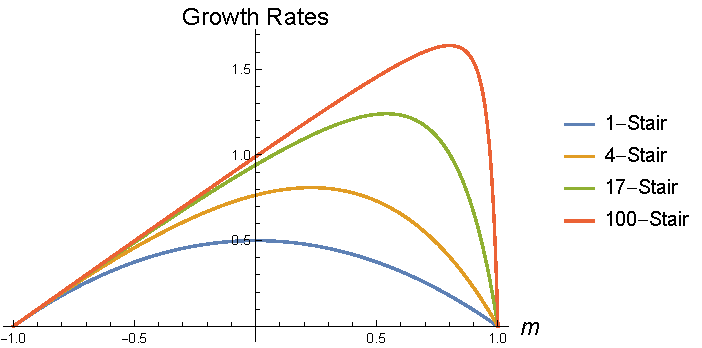
\includegraphics[width=.6\textwidth]{analrates}
	\caption{\textbf{Approximate growth rates} for 1-, 4-, 17-, and 100-stairs as a function of slope $m$. As stair length increases, the growth rate asymptotes to the function $\pd{S}{t} = m+1$.}
	\label{fig:growthrates}
\end{figure}

\subsubsection{Infinite Stairs}

Note that with increasing stair length the last term takes over and the growth rate asymptotes to the function $\Gamma_\infty = \gamma(m+1)$. This is the most asymmetric behavior, with the ratio $v_{B+}/v_{B-}$ increasing without limit. Furthermore $v_{B-}/v_E$ approaches 1 from above, and $v_{B+}/v_E$ increases without bound.

There are two ways to reason about this behavior. The first, which matches the order of limits of the current reasoning, is to start with infinite spatial support, which we have been assuming, and take the stair length $n\to\infty$. 
Alternatively, start with a finite spin chain with length $N$ and periodic boundary conditions, and set the stair length to $\infty$. Now a single gate acts on site $1,2,3\dots N$, before wrapping around to act at site 1 again. 

In both cases the rates $\Gamma_\infty(0)=\gamma$ and $\Gamma_\infty(1) = 2\gamma$ can be understood easily. In the $m=0$ case, after a gate falls between sites $i$ and $i+1$, $s_{i+1}$ will be a down slope regardless of whether the gate generated entanglement. Then the next gate falls across sites $i+1$ and $i+2$. At site $i+2$ $s_{i+2}=u$ with probability $\half$, so on average $\half$ of the gates produce 2 units of entanglement. At near-maximal slope nearly all slopes are $u$, except at the site to the right of the most recent gate. Then the next gate falls at a local minimum with probability 1, and all gates produce 2 units of entanglement.

Interestingly, this argument applies regardless of correlations, so that while the growth rates in this section are only approximate for finite $n>1$, the approximation actually becomes better at very large $n$. The only argument might be that if a long stair falls across multiple down steps, it will not generate the maximal entanglement and the sharp peak in $\Gamma_\infty = \gamma(m+1)$ might be rounded out. However, the earlier argument that these particles are uncorrelated means that the in the large $m$ limit the particles do not interact.

\subsubsection{Entanglement and Butterfly Velocities} \label{susub:vels}

The entanglement velocity can be immediately read from the entanglement growth rate. Again ignoring the correlations, it is just 
\begin{align}
v_E=\Gamma_n(0)=\frac{\gamma}{n}\left(n+\th{2^n}-1\right),
\end{align}
which starts at .5 at $m=0$ and asymptotes to 1, as it should. Since there is no way to define asymmetric entanglement velocities this is as far as we will take the analysis of $v_E$.

In these models we can extract asymmetric butterfly velocities, by looking at the slopes of $\Gamma_n(m)$ at $m=\pm 1$. The left-moving butterfly velocity, $v_{B-}$ stays constant with respect to $n$, while the right moving $v_{B+}$ increases without bound. The interpretation of these behaviors comes from Sec.~\ref{sub:coarse}, using the speed of operator edges. If a long stair falls across an operator's left edge, it can only move the edge one site, since by the time it moves the edge the next gate already acts farther right. However whenever a staircase hits a right edge it moves the edge to the end of the staircase, which in the large $n$ limit is arbitrarily far.

Since the operator edge dynamics are equivalent to down step ``particle" dynamics, we can discuss the latter, which is more directly related to $\Gamma(m)$.
For $n\to\infty$, in a system of length $L$, the maximal growth rate occurs when the slope is near-maximal, with only a single down step. This corresponds to a slope of $\frac{L-2}{L}$. Then with only a single local minimum in the entropy function, the local minimum moves one site to the right with each gate. Every gate that acts raises the entropy, resulting in an entropy gain of 2 per gate. Of course for a slope of 1, there is still no entropy generation.

If there are 2 down steps, for a slope of $\frac{L-4}{L}$, the entropy generation is almost the same. One local minimum still moves to the right with the leading edge of the staircase. However, once per staircase (once every $L$ gates), one down step is next to the other down step. This results in no entropy growth for that step, for an average entropy gain of $2\frac{L-1}{L}$.

This pattern continues as the slope decreases. With $\rho L$ down steps, the slope is $\frac{L-2\rho L}{L}$ and the average growth rate is $2\frac{L-\rho L}{L} = m+1$. At $m = -1$ there is no growth, as expected. At $m=0$, the growth rate is 1. This matches the discussion in Sec.~\ref{subsub:largestairs}.

When we combine left and right stairs to recover symmetry, in the limit of large $n$, the entanglement growth rate becomes $\Gamma(m)\to 1$, with $\Gamma(1) = \Gamma(-1)=0$. Since the slopes at $m=\pm1$ become infinite, these slopes have arbitrarily high $v_B/v_E$, which was shown using these symmetric staircase circuits in Ref.~\cite{Nahum2018}.

\subsection{Steady States with Correlation} \label{sub:steadystate}

The first correction to make to the previous section is to incorporate a non-zero correlation in the steady state. For example, the system could be slightly ferromagnetic or antiferromagnetic, meaning that after an up slope the next slope is slightly more or less likely to be up, respectively. These terms are used in analogy with the Ising model; there is no actual magnetism in the circuit. An antiferromagnetic state has more local minima, so more gates will generate entanglement leading to a higher growth rate.

The correlation affects the growth rate for 2-stairs through the probabilities in table~\ref{tab:2stair}. In a system with non-zero correlation they depend on both the slope and correlation, as shown below. We then show how to find the steady state in Secs.~\ref{subsub:randstate} and~\ref{subsub:stairstate}.

When looking at a single site, the probabilities of $u$ or $d$ are simple: $p(u) = \frac{1+m}{2}, p(d) = \frac{1-m}{2}$. Previously we used the na\"ive assumption that, when looking at 2 sites, $p(uu) = p(u)p(u)$. However this is only true without correlations. The nearest neighbor correlation $C_{i,i+1}$ completely captures this dependence. Since our system is translationally invariant, the correlation cannot depend on position so $C_{i,i+1}=C_1$.

Ignoring finite-size effects, we have
\begin{align}
\ex{s_is_{i+1}} &= p(uu) + p(dd) - p(ud) - p(du),\nn
m &= p(uu) - p(dd)\nn
C_{1} &= \ex{s_is_{i+1}}-\ex{s_i}\ex{s_{i+1}} = \ex{s_is_{i+1}} - m^2,\nn
&= p(uu) + p(dd) - p(ud) - p(du) - (p(uu))^2 - (p(dd))^2 + 2p(uu)p(dd).
\end{align}
Along with the constraint $p(ud)=p(du)$ due to the fact that their must be an even number of domain walls, this gives 4 constraints on 4 probabilities, so the 2-site probabilities are completely constrained.
After more manipulation we arrive at 
\begin{align}
p(ud) &= p(du) = \frac{1-m^2-C_1}{4},\\
p(uu) &= \frac{(1+m)^2+C_1}{4},\\
p(dd) &= \frac{(1-m)^2+C_1}{4}.
\end{align}
These reduce to our old expressions for $C_1\to0$.

If there were correlation in the random circuit then these new probabilities would affect the growth rate. However, as we will show, there is no correlation in that architecture. However, we can use $C_1$ to calculate the first order correction to the 2-stair growth rate. 

Referring back to table~\ref{tab:2stair}, the only quantities that have changed are the probabilities. Although we haven't explicitly calculated the 3-site probabilities, we can get the $C_1$ correction using Bayes' rule. For example,
\begin{align}
p(ddu) &= p(dd)*p(u|d) = p(dd)\frac{p(du)}{p(d)}\nn
&= \frac{(1-m)^2+C_1}{4}\frac{1-m^2-C_1}{4}\frac{2}{1-m}\nn
&= \frac{\left((1-m)^2+C_1\right) \left(1-m^2-C_1\right)}{8 (1-m)},
\end{align}
where $p(u|d)$ is the probability that $s_i=u$ given $s_{i-1}=d$.
This value is the same as it would be if we had started from the right side and calculated $p(ddu) = p(du)*p(d;d)$, where $p(d;d)$ is the probability that $s_i=d$ given $s_{i+1}=d$.

After calculating the other relevant probabilities and going through the same process used to generate Eq.~\ref{eqn:2rate}, we find
\begin{align}
\Gamma_2^{(1)}(m)=\frac{\gamma}{2}\frac{\left(1-m^2-C_1\right) \big((1+m) (5+m)
	\big)+C_1}{4 (1+m)},
\end{align}
which reduces to Eq.~\ref{eqn:2rate}.
The superscript notes that this is the $C_1$ correction to the growth rate. The $n$-stair growth rate will have corrections from correlations up to $C_n$. The analysis of these corrections will proceed similar to the analysis for $C_1$.

\subsubsection{Ergodicity and Stability} \label{subsub:ergstab}

To describe the steady state and extract a correlation we use the language of Markov processes. A Markov process is one in which the future state depends only on the current state, not the past. Label the states $s_i$ and define $p_{i,t}$ as the probability that the system is in state $s_i$ at time $t$. When there is a constant probability $S_{ij}$ of transitioning from state $j$ to state $i$ it is possible to write the transition matrix $S$ such that $p_{i,t+1}= S_{ij}p_{j,t}$. Since the product of the transition matrix and a probability vector gives the probabilities at the next time step, the transition matrix for $t$ time steps is just $S^t$. Under certain conditions the multi-step transition matrix approaches a constant matrix with all columns equal to the same vector $v^*$,
\begin{align}
\lim\limits_{t\to \infty}S^t = S^* = \begin{bmatrix}
\vdots & \vdots &  & \vdots\\
p^* & p^* & \cdots & p^*\\
\vdots & \vdots &  & \vdots\\
\end{bmatrix}.
\end{align}
Then the probability after a long time is the vector $p^*$ for any initial state.

The transition matrix can also be written as $S = 1+T$. The columns of $T$ must sum to 0 to preserve probabilities. From $S^*p^* = p^*,$ it must be true that $Tp^*=0$. This definition provides an easier route to finding $p^*$.

\subsubsection{Stable State in Random Architecture}  \label{subsub:randstate}

This analysis can be used to find the correlations present in the steady states of staircase architectures. Consider the 1-stair circuit, and enumerate 2-site (3-cut) states by the slope at the 2 sites: $s_1 = d\,d,\; s_2 = d\,u$, etc. Since at every time step there is an equal probability of a gate falling at any site, the transition matrix is the matrix product of single-cut transition matrices $P_{N} = \prod_NP_{1}\otimes$, where the 2-site transition matrix is 
\begin{align}
P_1 = \begin{bmatrix}
1-\frac{1+m}{2}\Gamma & 0      & \frac{1-m}{2}\Gamma & 0\\
\frac{1+m}{2}\Gamma & 1-\Gamma & 0                   & \frac{1-m}{2}\Gamma\\
0                   & \Gamma   & 1-\Gamma            & 0\\
0                   & 0        & \frac{1+m}{2}\Gamma & 1 - \frac{1-m}{2}\Gamma
\end{bmatrix}. \label{eqn:1sitetrans}
\end{align}
The $m$ dependence comes from the possibility of a gate acting on the left or right cut, which depends on the probability of the next slope being up or down.
The equilibrium state is
\begin{align}
v^* = \begin{pmatrix}
\frac{(1-m)^2}{4} \\ 
\frac{1+m}{2}\frac{1-m}{2} \\
\frac{1-m}{2}\frac{1+m}{2} \\
\frac{(1+m)^2}{4}
\end{pmatrix} = \begin{pmatrix}
\frac{1-m}{2} \\ \frac{1+m}{2}
\end{pmatrix} \otimes \begin{pmatrix}
\frac{1-m}{2} \\ \frac{1+m}{2}
\end{pmatrix},
\end{align}
which is uncorrelated, showing that the assumption of lack of correlation (used in equation~\ref{eqn:1sitetrans}) is consistent. Markov's theorem states that if all states are reachable from all other states\footnote{Probably introduce this earlier.} then the system is ergodic. An ergodic system contains only one equilibrium state, so the uncorrelated state is the unique equilibrium state.

\subsubsection{Stable States in Larger Staircases}  \label{subsub:stairstate}

Since the previous analysis relied on the assumption of lack of correlation and then showed its consistence, that will not work for larger stairs, which in fact do have a non-zero correlation. Instead of trying to calculate the correlation on an infinite system, which is complicated by having to know the previous and subsequent slopes, which rely on the correlation, we can find the steady state in small finite systems and extrapolate any measured quantities from these to large systems.

We do this by enumerating all possible states for our system of size $L$ and slope $m$ and building a transition $T$ matrix between states. Since gates have an equal probability of landing on each set of $n$ sites, the transition matrix element $T_{ij}$ will be $1/L$ times the number of ways state $i$ can be obtained after state $j$ using a single $n$-stair. Then the eigenvector of this matrix with eigenvalue 1 will be the steady state.

The hard part is constructing the transition matrices. For small systems it is possible to explicitly enumerate all states and calculate the probabilities of transitioning to other states from these. Luckily it is possible to calculate transition matrices for larger systems recursively from the small case. This step is made easier by calculating the matrices for all slopes, not just a specific one. we can then take only the subspace of slope $m$. We will go through this procedure for 2-stairs.

The case for $L=2$ is almost trivial. There are 4 states: $dd$, $du$, $ud$, $uu$. Recall that the systems are periodic, so for example the first state would look like $dddddd\dots$ if viewed over multiple periods. The first and last state have no local minima, so gates cannot change the states and these are stationary. For the middle two states, label the cut before the listed sites cut 0 and the cut between the listed sites cut 1. Then for the state $du$ cut 0 is a local maximum and cut 1 is a local minimum. If the first gate in the two stair lands on cut 1, the state will become $ud$, and will finish in state $du$ after the second gate. Otherwise the first gate, on cut 0, will have no effect and the final state will be $ud$, after the second gate falls on the local minimum. State $ud$ has a similar analysis. The result is that from either $m=0$ state, the probability of transition to the either $m=0$ state is $1/2$.

The 2-site transition matrix for 2-stairs is then 
\begin{align}
T_{2,2} &= 
\half \begin{bmatrix}
	2 & 0 & 0 & 0 \\
	0 & 1 & 1 & 0 \\
	0 & 1 & 1 & 0 \\
	0 & 0 & 0 & 2
	\end{bmatrix}
\end{align}
The steady state for $m=1$ is $uu$, the steady state for $m=-1$ is $dd$, and the steady state for $m=0$ is $\half(ud+du)$. The result that steady states for extremal slopes are all up or all down is general.

For the 3-site transition matrix we will show the calculation of 2 columns and then display the full matrix. Once again the state $ddd$ cannot transition, so the first column is $(1,0,0\dots)$. The second state in our basis is $ddu$, with $m=-1/3$. If the two gates fall on cuts 0 and 1, there is no change. If they land on cuts 1 and 2 or on sites 2 and 3 the final state is $dud$. These three possibilities are shown in Fig.~\ref{fig:3trans}.
\begin{figure}
	\centering
	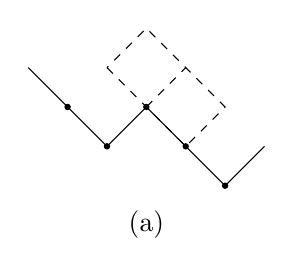
\begin{tikzpicture}
[scale = .5, dot/.style ={draw,shape=circle, fill=black, scale=.2}]
\draw (0,0) -- (1,-1) node[dot]{} -- (2,-2) node[dot]{} -- (3,-1) node[dot]{} --
      (4,-2) node[dot]{} -- (5,-3) node[dot]{} -- (6,-2);
\draw[dashed] (2,0) -- (4,-2) -- (5,-1) -- (3,1) -- (2,0) (3,-1) -- (4,0);
\draw (3,-4) node{(a)};
\end{tikzpicture}
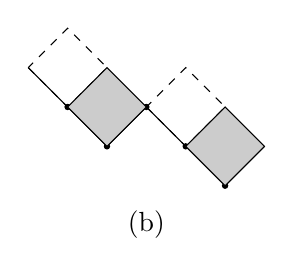
\begin{tikzpicture}
[scale = .5, dot/.style ={draw,shape=circle, fill=black, scale=.2}]
\draw (0,0) -- (1,-1) node[dot]{} -- (2,-2) node[dot]{} -- (3,-1) node[dot]{} --
(4,-2) node[dot]{} -- (5,-3) node[dot]{} -- (6,-2);
\draw[dashed] (0,0) -- (1,-1) -- (2,0) -- (1,1) -- (0,-0);
\draw[fill=black!20] (1,-1) -- (2,-2) -- (3,-1) -- (2,0) -- (1,-1);
\draw[dashed] (3,-1) -- (4,-2) -- (5,-1) -- (4,0) -- (3,-1);
\draw[fill=black!20] (4,-2) -- (5,-3) -- (6,-2) -- (5,-1) -- (4,-2);
\draw (3,-4) node{(b)};
\end{tikzpicture}
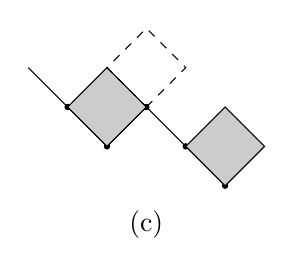
\begin{tikzpicture}
[scale = .5, dot/.style ={draw,shape=circle, fill=black, scale=.2}]
\draw (0,0) -- (1,-1) node[dot]{} -- (2,-2) node[dot]{} -- (3,-1) node[dot]{} --
(4,-2) node[dot]{} -- (5,-3) node[dot]{} -- (6,-2);
\draw[fill=black!20] (1,-1) -- (2,-2) -- (3,-1) -- (2,0) -- (1,-1);
\draw[dashed] (3,-1) -- (4,0) -- (3,1) -- (2,0) -- (3,-1);
\draw[fill=black!20] (4,-2) -- (5,-1) -- (6,-2) -- (5,-3) -- (4,-2);
\draw (3,-4) node{(c)};
\end{tikzpicture}
	\caption{\textbf{Three possible transitions} from the state $ddu$. Two different gate configurations result in the state $dud$. Recall that the system is periodic.}
	\label{fig:3trans}
\end{figure}
Both final states have $m=-1/3$, since all final states have to have the same slope as the initial state. This is what allows us to decompose the full transition matrix into subspaces. 

The full 3-site, 2-stair transition matrix is
\begin{align}
T_{2,3} = 
\th{3}\begin{bmatrix}
	3 & 0 & 0 & 0 & 0 & 0 & 0 & 0\\
	0 & 1 & 0 & 0 & 2 & 0 & 0 & 0\\
	0 & 2 & 1 & 0 & 0 & 0 & 0 & 0\\
	0 & 0 & 0 & 1 & 0 & 1 & 1 & 0\\
	0 & 0 & 2 & 0 & 1 & 0 & 0 & 0\\
	0 & 0 & 0 & 1 & 0 & 1 & 1 & 0\\
	0 & 0 & 0 & 1 & 0 & 1 & 1 & 0\\
	0 & 0 & 0 & 0 & 0 & 0 & 0 & 3
	\end{bmatrix}
\end{align}
There are two keys to building the larger transition matrices. First, instead of the transition matrix for gates at all 3 cuts, we can look at only transitions due to gates on cuts 1 and 2,
\begin{align}
T_{2,3}^{(1)} =
\begin{bmatrix}
	1 & 0 & 0 & 0 & 0 & 0 & 0 & 0\\
	0 & 0 & 0 & 0 & 0 & 0 & 0 & 0\\
	0 & 1 & 0 & 0 & 0 & 0 & 0 & 0\\
	0 & 0 & 0 & 0 & 0 & 0 & 0 & 0\\
	0 & 0 & 1 & 0 & 1 & 0 & 0 & 0\\
	0 & 0 & 0 & 0 & 0 & 0 & 0 & 0\\
	0 & 0 & 0 & 1 & 0 & 1 & 1 & 0\\
	0 & 0 & 0 & 0 & 0 & 0 & 0 & 1
	\end{bmatrix}
\end{align}
The other 2 components of the transition matrix will be this matrix, with states permuted by 1 or two spaces. This permutation can be achieved using the cyclic swap matrix $S_3$ from Sec.~\ref{sec:asymham}, so that $T_{2,3}^{(2)}=S_3\,T_{2,3}^{(1)}\,S_3^{-1}$, etc.

The usefulness of this decomposition comes when looking at the analogous matrix for 4 sites,
%\begin{align}
%T_{2,4}^{(1)} =
%\left[
%\begin{array}{cccccccccccccccc}
%1 & 0 & 0 & 0 & 0 & 0 & 0 & 0 & 0 & 0 & 0 & 0 & 0 & 0 & 0 & 0 \\
%0 & 1 & 0 & 0 & 0 & 0 & 0 & 0 & 0 & 0 & 0 & 0 & 0 & 0 & 0 & 0 \\
%0 & 0 & 0 & 0 & 0 & 0 & 0 & 0 & 0 & 0 & 0 & 0 & 0 & 0 & 0 & 0 \\
%0 & 0 & 0 & 0 & 0 & 0 & 0 & 0 & 0 & 0 & 0 & 0 & 0 & 0 & 0 & 0 \\
%0 & 0 & 1 & 0 & 0 & 0 & 0 & 0 & 0 & 0 & 0 & 0 & 0 & 0 & 0 & 0 \\
%0 & 0 & 0 & 1 & 0 & 0 & 0 & 0 & 0 & 0 & 0 & 0 & 0 & 0 & 0 & 0 \\
%0 & 0 & 0 & 0 & 0 & 0 & 0 & 0 & 0 & 0 & 0 & 0 & 0 & 0 & 0 & 0 \\
%0 & 0 & 0 & 0 & 0 & 0 & 0 & 0 & 0 & 0 & 0 & 0 & 0 & 0 & 0 & 0 \\
%0 & 0 & 0 & 0 & 1 & 0 & 0 & 0 & 1 & 0 & 0 & 0 & 0 & 0 & 0 & 0 \\
%0 & 0 & 0 & 0 & 0 & 1 & 0 & 0 & 0 & 1 & 0 & 0 & 0 & 0 & 0 & 0 \\
%0 & 0 & 0 & 0 & 0 & 0 & 0 & 0 & 0 & 0 & 0 & 0 & 0 & 0 & 0 & 0 \\
%0 & 0 & 0 & 0 & 0 & 0 & 0 & 0 & 0 & 0 & 0 & 0 & 0 & 0 & 0 & 0 \\
%0 & 0 & 0 & 0 & 0 & 0 & 1 & 0 & 0 & 0 & 1 & 0 & 1 & 0 & 0 & 0 \\
%0 & 0 & 0 & 0 & 0 & 0 & 0 & 1 & 0 & 0 & 0 & 1 & 0 & 1 & 0 & 0 \\
%0 & 0 & 0 & 0 & 0 & 0 & 0 & 0 & 0 & 0 & 0 & 0 & 0 & 0 & 1 & 0 \\
%0 & 0 & 0 & 0 & 0 & 0 & 0 & 0 & 0 & 0 & 0 & 0 & 0 & 0 & 0 & 1 \\
%\end{array}
%\right]
%\end{align}
The second key is that this is just $T_{2,3}^{(1)}\otimes I_2$. This is because gates on the cuts 1 and 2 only affect the first 3 slopes. Since the computational basis is arranged such that $ddud$ is immediately followed by $dduu$, each $2\times 2$ block of a larger matrix is the identity times the corresponding element of the smaller matrix.

We can now build the full $T_{2,4}$ from $T_{2,4}^{(1)}$ and its permutations. From subspaces of constant slope we can find the steady states, for example the $m=0$ steady state
\begin{align}
s_{m=0} = \th{5}dduu + \th{10}dudu + \th{5} duud + \th{5}uddu + \th{10}udud + \th{5}uudd.
\end{align}

Given the steady state it is possible to calculate the steady state correlation by averaging the correlations in each component of the steady state, weighted by their coefficients. The only hitch here is that the obvious formula for correlation, $C_1 = \ex{s_is_{i+1}}-\ex{s_i}^2$ does not work for finite systems if the expectations are interpreted as averages.  To see why, consider a 6-site state with slope 0. If the first 3 slopes are up, the last 3 have to be down to maintain the state. This introduces a negative bias into the overall correlation, equal to $1/(L-1)$, where $L$ is the length of the system. 

It is possible to correct for this bias by adding back the bias, so the true correlation of, for example, the state $uududu$ is 
\begin{align}
C_1 &= \ex{s_is_{i+1}} - \ex{s}^2 + \th{L-1}\nn
&= \frac{1-1-1-1-1+1}{6} - \frac{2^2}{6^2} + \th{6-1}\nn
&= -\frac{1}{3} - \frac{1}{9} + \th{5}\nn
&= -\frac{11}{45}.
\end{align}
After repeating this calculation for other states we can find the steady states in various size systems. For $m=0$, these are
\begin{align}
L=4, \qquad &C_1=0.1333\nn
L=6, \qquad &C_1=0.1103\nn
L=8, \qquad &C_1=0.1171\nn
L=10,\qquad &C_1=0.1163.
\end{align}
To actually show that the correlation asymptotes to a value we would have to take these calculations out to very large $L$. However, we can see now that the correlation will be positive and $\approx0.11$ or $0.12$. 

For nonzero $m$ we have fewer choices of $L$. For example, for $m=\pm\th{2}$, $L$ must be a multiple of 4. The steady state correlations for $m=\th{2}$ are
\begin{align}
L = 4, \qquad &C_1=0.0833\nn
L = 8, \qquad &C_1=0.0760\nn
L =12, \qquad &C_1=0.0703,
\end{align}
while for $m=-\half$,
\begin{align}
L = 4, \qquad &C_1=0.0833\nn
L = 8, \qquad &C_1=0.1151\nn
L =12, \qquad &C_1=0.1017.
\end{align}
The relevant information here is that both correlations are smaller than at $m=0$, but the correlation is significantly larger in the negative slope system.\footnote{why?}

\subsection{Numerical Simulation} \label{sub:num}

To simulate the entropy growth in infinite spin chains with non-zero slope, we use finite chains with periodic boundary conditions, where one end of the chain is attached to the other with an offset. The spin chains are initialized with an uncorrelated entanglement function with each slope chosen to be up or down with $p(u)=(1+m)/2$. This results in a sample slope that is near the given slope. Then, for each time step, a random gate location is chosen. The entanglement across that cut, and the next $n-1$, is calculated using the update rule from Eq.~\ref{eqn:update}.

Since larger gates will generate non-zero correlation, the initial $S(x)$ is not a valid steady state. However the dynamics should bring the system into a steady state, so growth rates are calculated for only the latter part of the simulation. Fig.~\ref{fig:corrgrowth} shows that there is a time after which the correlations reach this steady state.

\subsubsection{Measuring Growth Rates}  \label{subsub:growthrates}

To calculate the growth rates we start in the initial uncorrelated state and evolve with 400 $n$-stairs, then average the growth rate over the next 1600 stairs. This procedure is repeated 100 times to calculate statistics on the mean. Growth rates for stairs of various lengths are shown in Fig.~\ref{fig:compareRates}. As length increases, the growth rate follows the same pattern as predicted, increasing with the maximum moving right. 
\begin{figure}
	\centering
	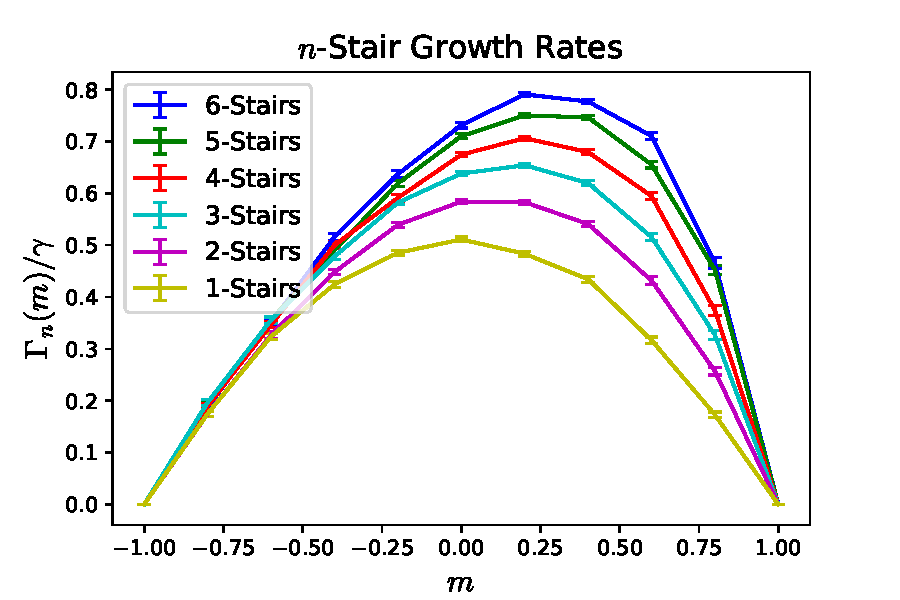
\includegraphics[width=.5\textwidth]{compareRates.pdf}
	\caption{\textbf{Growth rates for different length stairs.} All growth rates were calculated using a 100-site spin chain with offset periodic boundary conditions. Rates were calculated from the application of 2,000 gates total, or 20 per site, averaged over the last 80\% of the gates in order to build up correlations, then averaged over 100 trials.}
	\label{fig:compareRates}
\end{figure}

For 1-stairs (the random architecture), the measured growth rate is not significantly different than predicted, seen in Fig.~\ref{fig:1stairRates}.
\begin{figure}
	\centering
	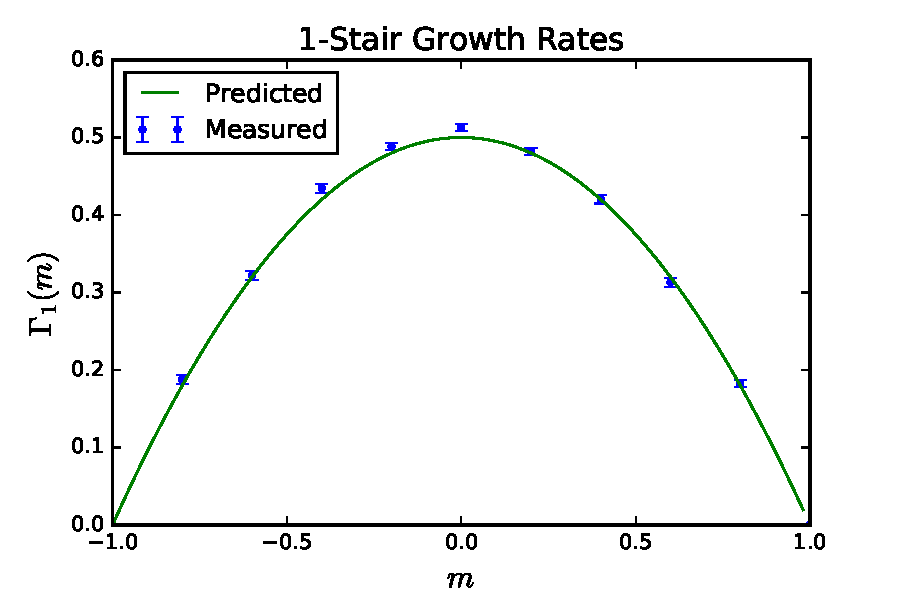
\includegraphics[width=.5\textwidth]{1stairRates.pdf}
	\caption{\textbf{Measured and analytic growth rates} for the 1-stair architecture. Note that the measured rate is not different than predicted.}
	\label{fig:1stairRates}
\end{figure}
This implies that the lack of correlation is exact, and that the finite size effects are small enough at $L=100$ to not significantly affect $\Gamma_1(m)$.

Stairs of length greater than 1 do however generate correlations. Figure~\ref{fig:6stairRates} shows the growth rates for 6-stairs. 
\emph{Normalized}
\emph{Does this go away?}
\begin{figure}
	\centering
	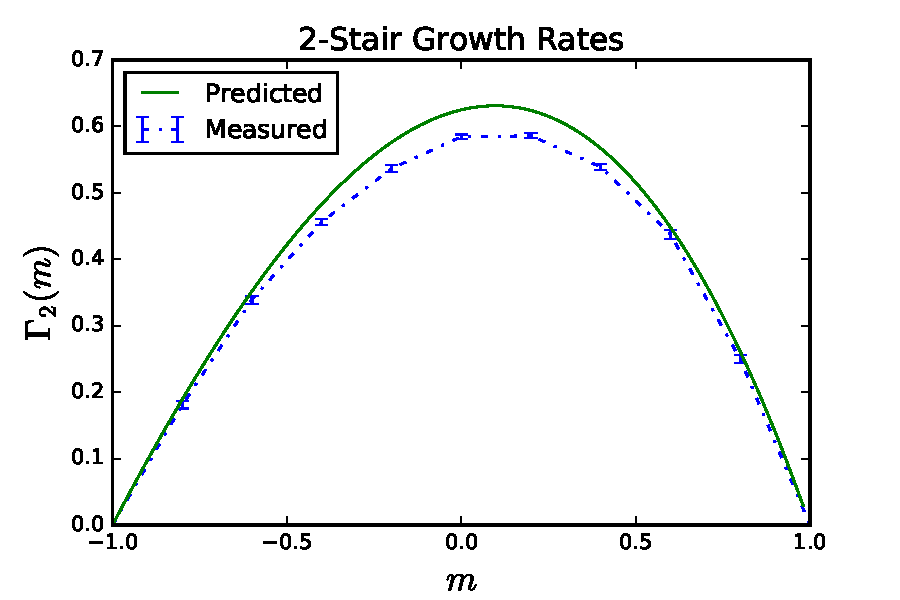
\includegraphics[width=.495\textwidth]{2stairRates.pdf}
	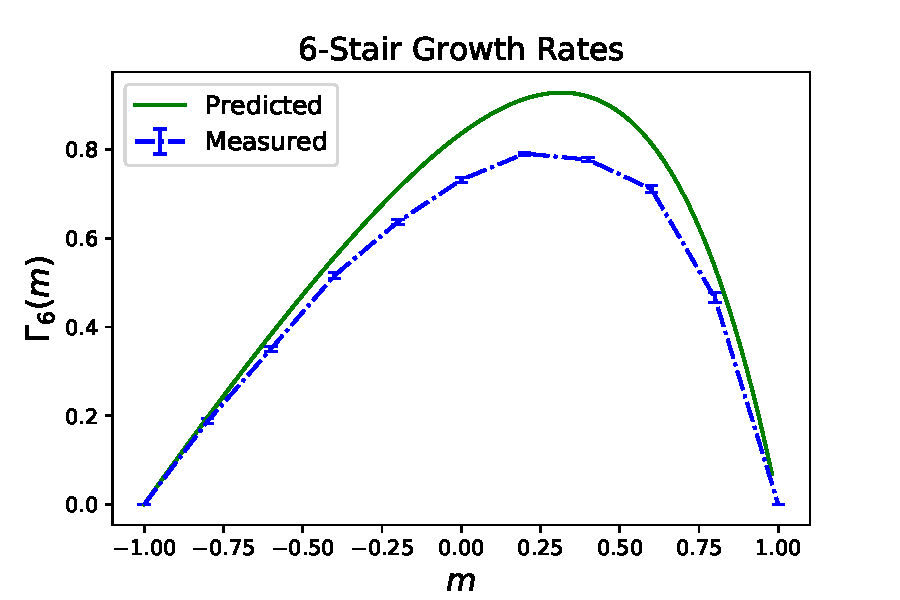
\includegraphics[width=.495\textwidth]{6stairRates.pdf}
	\caption{\textbf{Measured and predicted growth rates} for the 2- and 6-stair architecture. The measured rate is now significantly lower than predicted, implying that the correlations built up by the stairs act to lower their entropy production.}
	\label{fig:6stairRates}
\end{figure}
The notable difference in growth rate here is probably due to correlations created by the 6-stairs. Hopefully reasoning similar to that in Sec.~\ref{sub:steadystate} will be able to predict the correlation so that its effect, at least to first order, can be calculated. This would allow a much closer approximation than that in Fig.~\ref{fig:6stairRates}

\subsubsection{Measuring Correlations}  \label{subsub:correlations}

In Sec.~\ref{sub:steadystate} we found the correlation in the steady state \_\_\_\_\_\_. We can check this numerically, by initializing a state with 0 correlation, evolving it, and measuring the correlation at later times. In general the correlation grows to the steady state value and then levels off. Fig.~\ref{fig:corrgrowth} shows the evolution of the correlation in 1- 2- 3- and 10-stair circuits, averaged over 40 trials.
\begin{figure}
	\centering
	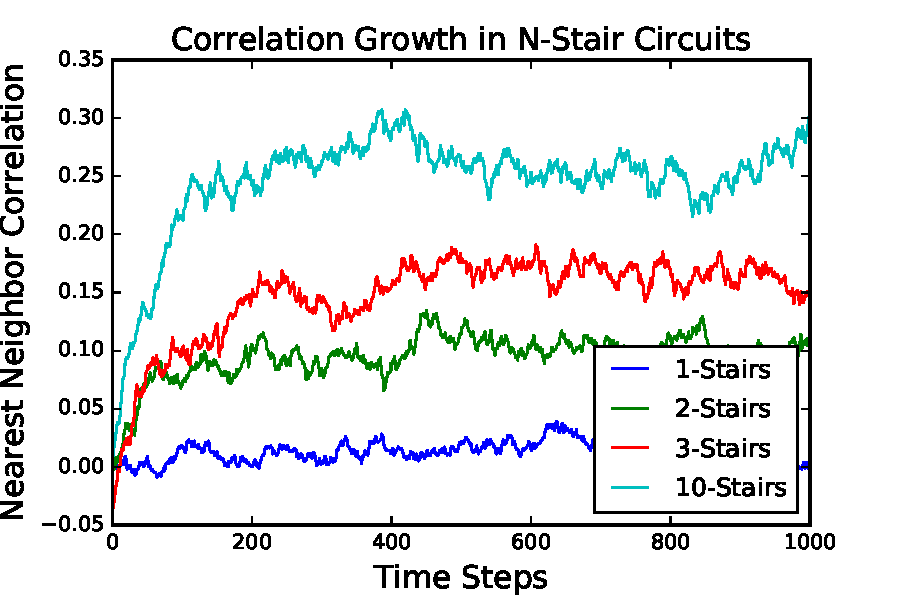
\includegraphics[width=.5\textwidth]{Ncorrgrowth.pdf}
	\caption{\textbf{Correlation Growth for 0 slope.} Each curve corresponds to an initially 0 entanglement curve evolved with the given circuit architecture. Time in this plot is normalized so that one time step corresponds to one N-stair. This way, all curves reach steady-state entanglement by about 400 steps.
	}
	\label{fig:corrgrowth}
\end{figure}
As expected, the random circuit produces no significant correlation. Larger stairs do, and this should be taken into account when calculating growth rates. 

The correlation also depends on the slope of the entanglement curve. This must be true because $C_1=0$ for $m=\pm1$, and the correlation should vary smoothly with slope. Figure~\ref{fig:steadystate} shows this dependence. All curves were created by first evolving by 400 time steps to remove the initial conditions, and then sampling \_\_\_\_ points, separated by \_\_\_\_ steps.
\begin{figure}
	\centering
	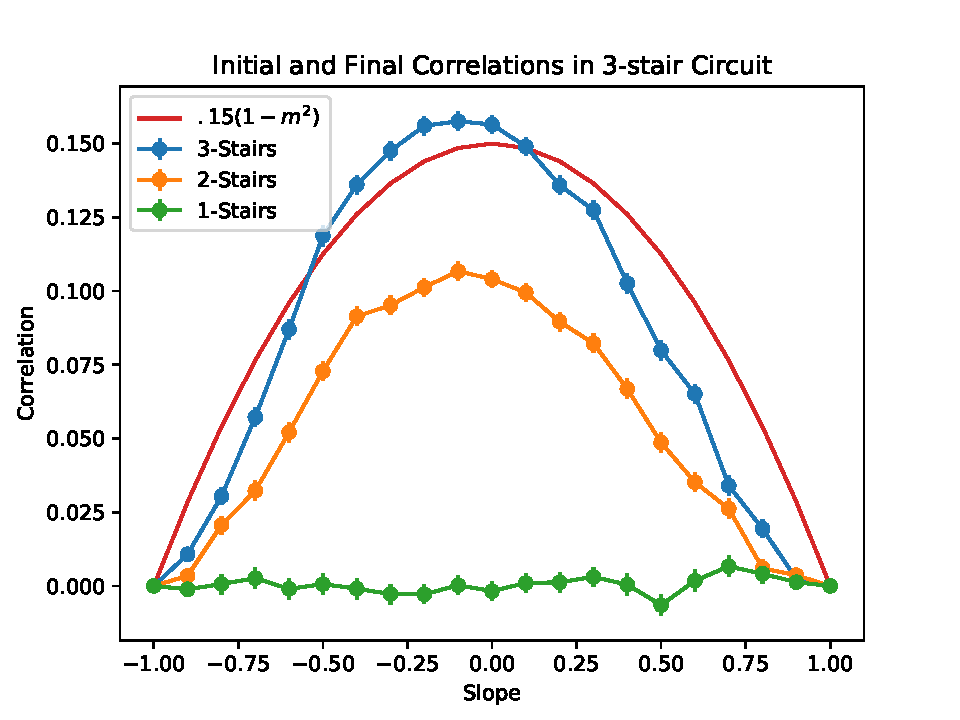
\includegraphics[width=.6\textwidth]{beststairCorrel.pdf}
	\caption{\textbf{Correlations created by 1-, 2-, and 3-stair circuits.} The correlation in 1-stair circuits is consistent with 0. Larger stairs generate significant correlation. The analytic function, $.15(1-m^2)$, acts as a guide to show that the correlations are asymmetric with respect to $m$.}
	\label{fig:steadystate}
\end{figure}

The 3-stair circuit indeed generates more correlation than the 1-stair circuit. The solid curve is a simple quadratic function of the slope, which shows that the correlation function is asymmetric, and that negative slope states have slightly more correlation in the steady state. \emph{Why?}

We can insert this empirical correlation into the growth rate correlation to get a closer estimate of the true growth rate. Fig.~\ref{fig:2corRates} compares this procedure to the earlier calculation. The systematic error appears to now be in the other direction, overestimating the growth rate of these circuits.
\emph{Relabel plots with better legends}
\begin{figure}
	\centering
	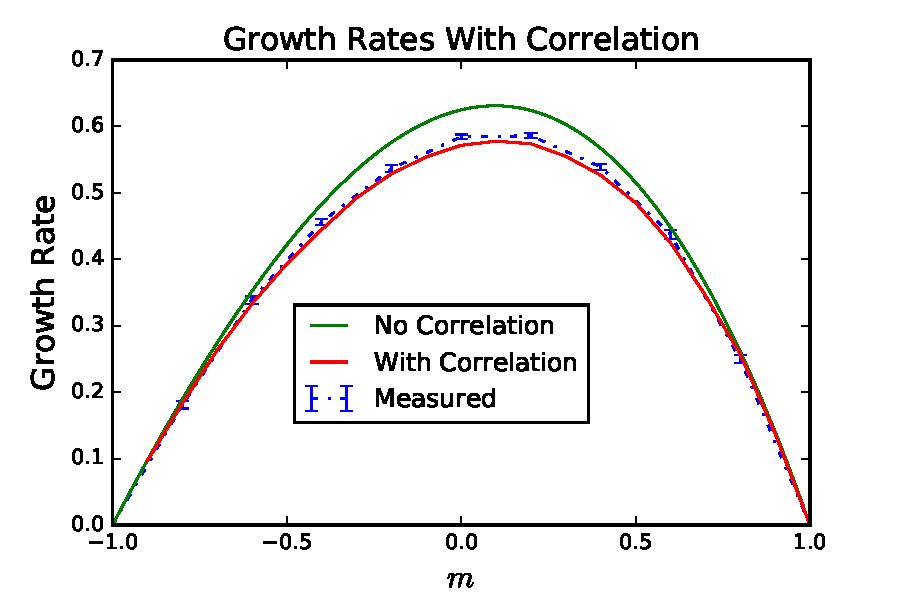
\includegraphics[width=.495\linewidth]{2corRates}
	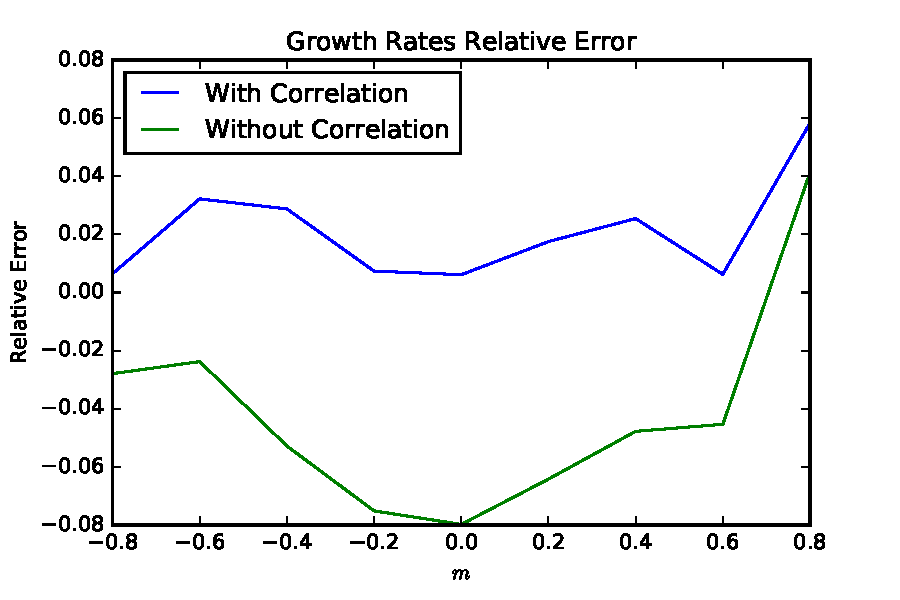
\includegraphics[width=.495\linewidth]{2corErrors}
	\caption{\textbf{Growth rates with and without correcting for non-zero correlation} in the steady state. Including the correlation removes a significant portion of the error.}
	\label{fig:2corRates}
\end{figure}

The nearest neighbor correlation is not the only correlation in the system. A given step can also be correlated with a step $\l$ sites away from it. Again because the system is translationally invariant this correlation is dependent on distance, and can be called $C_\l$. Since the $n$-stair architecture is itself highly correlated to a scale of $n$, it would be unsurprising if $C_\l$ was significantly for $\l\ge n$. 

Fig.~\ref{fig:cor_length} shows $C_\l$ for various circuit architectures. $C_\l$ is positive for $\l\ge n$, dips negative for the next few correlation lengths, and approaches 0 for long distance correlation.
\begin{figure}
	\centering
	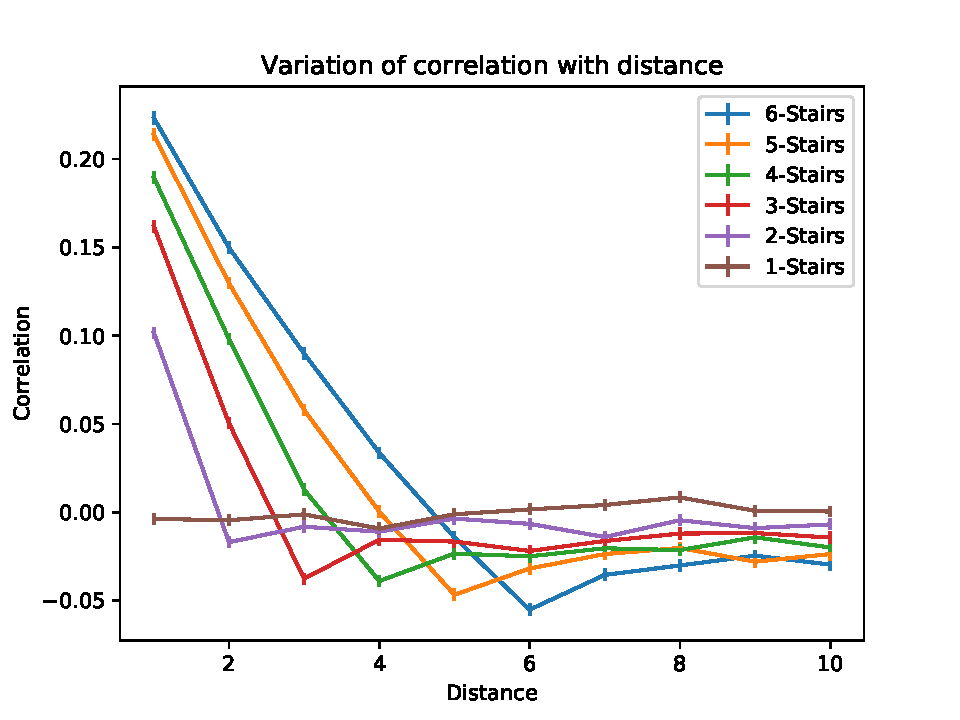
\includegraphics[width=.5\linewidth]{cor_length}
	\caption{\textbf{Variable-distance correlation for various architectures.} Note that the correlation is generally positive for $\l<n$, until $n=6$.}
	\label{fig:cor_length}
\end{figure}
This suggests that it might be possible to have a circuit architecture with a mix of staircases of different lengths, such that correlations introduced by different length stairs cancel each other out.

Instead of looking at the variation of correlation with respect to distance, we can look at variation with respect to stair length, as in Fig.~\ref{fig:cor_stair}.
\begin{figure}
	\centering
	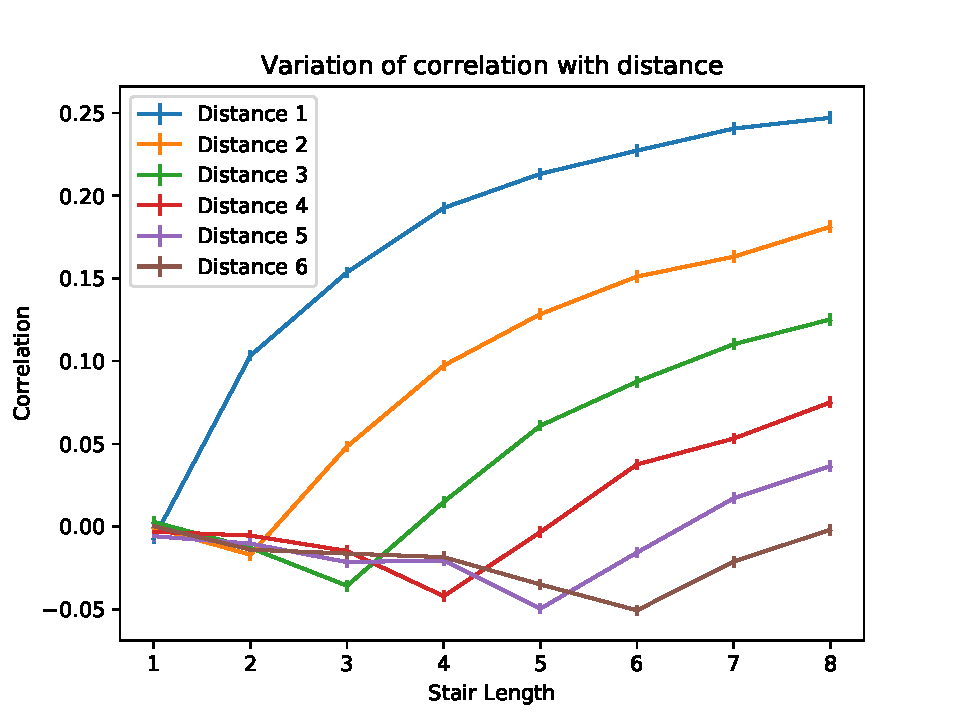
\includegraphics[width=.5\textwidth]{cor_stair}
	\caption{\textbf{Dependence of correlation on stair length} for different $\l$. Note that the correlation appears to level off for long stairs.}
	\label{fig:cor_stair}
\end{figure}
This does not include new information, but presents the information from Fig.~\ref{fig:cor_length} differently. In particular, it appears that the correlation begins to level off for large stairs. Once again, the negative correlation for $n\approx\l$ is assumed to be due to finite-size effects.